\section{ECEF}
Earth-Centered-Earth-Fixed coordinates belong to the easiest coordinates to compute, because they have a fixed frame and they don't have to regard the non-spherical shape of the earth. Though they are not intuitiv. \\
\begin{figure}[h!]
	\centering
	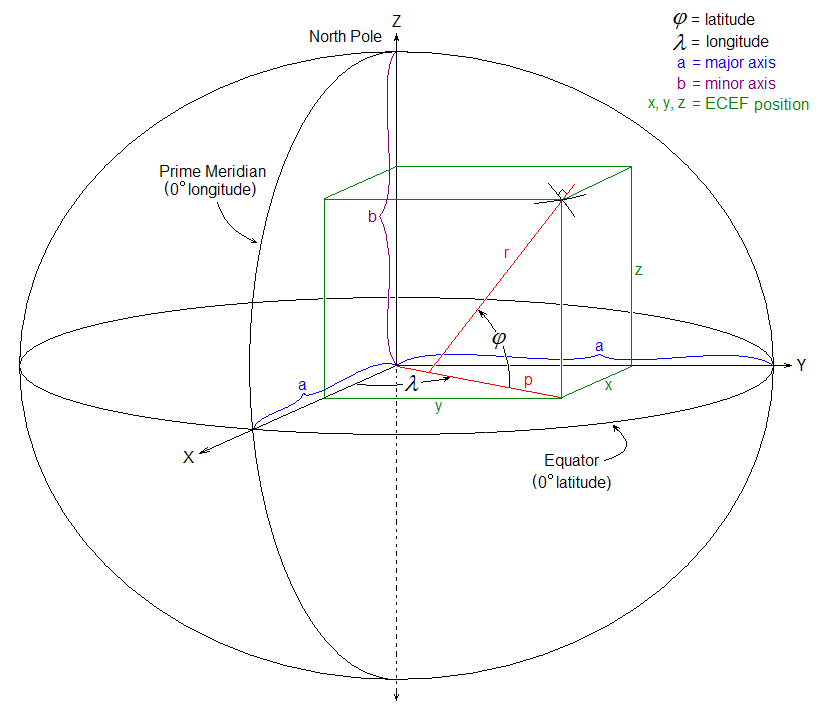
\includegraphics[width=10cm]{ECEF}
	\caption{ECEF coordinates}
	\label{ECEF coordinates}
\end{figure}

ECEF coordinates are defined using
\begin{equation}
p_{ECEF} = \begin{pmatrix} x \\ y \\ z \end{pmatrix}
\end{equation}
available for the following simple types
\begin{itemize}
\item int32\_t - \texttt{EcefCoor\_i}
\item float - \texttt{EcefCoor\_f}
\item double - \texttt{EcefCoor\_d}
\end{itemize}




\subsection{Transformations from ECEF}
\subsubsection*{to LTP}
Gets the LLA-coordinates and a transformation matrix from ECEF to ENU out of ECEF coordinates.

First, the LLA coordinates (WGS-84) are computed from the ECEF coordinates. 

With the LLA-coordinates it is possible to construct a rotational matrix.
\begin{equation}
\mat R_{ecef2enu} = \begin{pmatrix}
-\sin \lon				& \cos \lon				&		0	\\
-\sin \lat \cos \lon	& -\sin \lat \sin \lon	& \cos \lat	\\
\cos \lat \cos \lon		& \cos \lat \sin \lon	& \sin \lat	
\end{pmatrix}
\end{equation}
\inCfile{ltp\_def\_from\_ecef\_i(LtpDef\_i* def, EcefCoor\_i* ecef)}{pprz\_geodetic\_int}
\inCfile{ltp\_def\_from\_ecef\_f(LtpDef\_f* def, EcefCoor\_f* ecef)}{pprz\_geodetic\_float}
\inCfile{ltp\_def\_from\_ecef\_d(LtpDef\_d* def, EcefCoor\_d* ecef)}{pprz\_geodetic\_double}

\subsubsection*{to LLA}
Generating LLA coordinates is made using the following calculations. These refer to \cite{wiki:1} or \cite{Wendel__2007}(pages 31-33).

\begin{align}
a	&= 6,378,137										\\
f	&= \frac{1}{298.257223563}							
\end{align}
\begin{align}
b	&= a \multiplication (1-f)							\\
e^2	&= \sqrt{2f-f^2}									\\
e'	&= e \frac{a}{b}									\\
E^2	&= a^2-b^2											\\
r	&= \sqrt{ x^2 + y^2}								\\
F	&= 54 b^2 z^2										\\
G	&= r^2 + (1-e^2)z^2-e^2E^2							\\
c	&= \frac{e^4Fr^2}{G^3}								\\
s	&= \sqrt[3]{1+c+\sqrt{c^2+2c}}						\\
P	&= \frac{F}{3\left(s+\tfrac 1 s + 1\right)^2 G^2}	\\
Q	&= \sqrt{1+2e^4P}									\\
r_0	&= -\frac{Pe^2r}{1+Q} + \sqrt{\tfrac 1 2 a^2 \left(1 + \tfrac 1 Q \right) - \frac{P(1-e^2)z^2}{Q(1+Q)}-\tfrac 1 2 P r^2}	\\
U	&= \sqrt{(r-e^2r_0)^2+z^2}							\\
V	&= \sqrt{(r-e^2r_0)^2+(1-e^2)z^2}					\\
z_0	&= \frac{b^2z}{aV}									\\
\lat	&= \arctan \left( \frac{z+(e')^2z_0} r \right)	\\
\lon	&= atan2(y,x)									\\
h	&= U \left( \frac{b^2}{aV} - 1 \right)
\end{align}
\inCfile{lla\_of\_ecef\_i(LlaCoor\_i* out, EcefCoor\_i* in)}{pprz\_geodetic\_int}
\inCfile{lla\_of\_ecef\_f(LlaCoor\_f* out, EcefCoor\_f* in)}{pprz\_geodetic\_float}
\inCfile{lla\_of\_ecef\_d(LlaCoor\_d* lla, EcefCoor\_d* ecef)}{pprz\_geodetic\_double}

\subsubsection*{to NED/ENU}
With a know transformation matrix (see section \ref{LTP}) it is quite easy to rotate a vector into the ENU frame:
\begin{equation}
\vect v_{ENU} = \mat R_{ecef2enu} \vect v_{ECEF}
\end{equation}
For a transformation into the NED-frame you have to do an additional ENU/NED-transformation.

\inCfile{enu\_of\_ecef\_vect\_i(EnuCoor\_i* enu, LtpDef\_i* def, EcefCoor\_i* ecef)}{pprz\_geodetic\_int}
\inCfile{ned\_of\_ecef\_vect\_i(NedCoor\_i* ned, LtpDef\_i* def, EcefCoor\_i* ecef)}{pprz\_geodetic\_int}
\inCfile{enu\_of\_ecef\_vect\_f(EnuCoor\_f* enu, LtpDef\_f* def, EcefCoor\_f* ecef)}{pprz\_geodetic\_float}
\inCfile{ned\_of\_ecef\_vect\_f(NedCoor\_f* ned, LtpDef\_f* def, EcefCoor\_f* ecef)}{pprz\_geodetic\_float}
\inCfile{enu\_of\_ecef\_vect\_d(EnuCoor\_d* enu, LtpDef\_d* def, EcefCoor\_d* ecef)}{pprz\_geodetic\_double}
\inCfile{ned\_of\_ecef\_vect\_d(NedCoor\_d* ned, LtpDef\_d* def, EcefCoor\_d* ecef)}{pprz\_geodetic\_double}

The transformation of a point is very similiar. Instead of a point you use a difference vector between the desired point $p_d$ and the center of the local tangent plane $p_0$.
\begin{equation}
\vect v_{ECEF} = p_d - p_0
\end{equation}
\inCfile{enu\_of\_ecef\_point\_i(EnuCoor\_i* enu, LtpDef\_i* def, EcefCoor\_i* ecef)}{pprz\_geodetic\_int}
\inCfile{ned\_of\_ecef\_point\_i(NedCoor\_i* ned, LtpDef\_i* def, EcefCoor\_i* ecef)}{pprz\_geodetic\_int}
\inCfile{enu\_of\_ecef\_point\_f(EnuCoor\_f* enu, LtpDef\_f* def, EcefCoor\_f* ecef)}{pprz\_geodetic\_float}
\inCfile{ned\_of\_ecef\_point\_f(NedCoor\_f* ned, LtpDef\_f* def, EcefCoor\_f* ecef)}{pprz\_geodetic\_float}
\inCfile{enu\_of\_ecef\_point\_d(EnuCoor\_d* enu, LtpDef\_d* def, EcefCoor\_d* ecef)}{pprz\_geodetic\_double}
\inCfile{ned\_of\_ecef\_point\_d(NedCoor\_d* ned, LtpDef\_d* def, EcefCoor\_d* ecef)}{pprz\_geodetic\_double}


\subsection{Transformations to ECEF}
\subsubsection*{from LLA}
Calculating the ECEF coordinates out of LLA coordinates is a slightly easier task than the other way round. The following way refers to \cite{wiki:1}. With the known constants
\begin{align}
a	&= 6,378,137				\\
f	&= \frac{1}{298.257223563}	\\
e^2	&= \sqrt{2f-f^2}			
\end{align}
the value
\begin{equation}
\chi = \sqrt{1-e^2\sin^2 \lat}
\end{equation}
can be precomputed and used in
\begin{align}
x &= \left(\tfrac a \chi + h \right) \cos \lat \cos \lon \\
y &= \left(\tfrac a \chi + h \right) \cos \lat \sin \lon \\
z &= \left(\tfrac a \chi (1-e^2) + h \right) \sin \lat
\end{align}
\inCfile{ecef\_of\_lla\_i(EcefCoor\_i* out, LlaCoor\_i* in)}{pprz\_geodetic\_int}
\inCfile{ecef\_of\_lla\_f(EcefCoor\_f* out, LlaCoor\_f* in)}{pprz\_geodetic\_float}
\inCfile{ecef\_of\_lla\_d(EcefCoor\_d* ecef, LlaCoor\_d* lla)}{pprz\_geodetic\_double}

\subsubsection*{from NED/ENU}
With a know transformation matrix (see section \ref{LTP}) it is quite easy to rotate a vector from the ENU-frame to the ECEF-frame.
Since
\begin{equation}
\mat R_{enu2ecef} = \inv{\mat R_{ecef2enu}} = \transp{\mat R_{ecef2enu}}
\end{equation}
a transformation is done as follows
\begin{equation}
\vect v_{ECEF} = \mat R_{enu2ecef} \vect v_{ENU} 
\end{equation}
For a transformation from the NED-frame you have to do an additional ENU/NED-transformation before.

\inCfile{ecef\_of\_enu\_vect\_d(EcefCoor\_d* ecef, LtpDef\_d* def, EnuCoor\_d* enu)}{pprz\_geodetic\_double}
\inCfile{ecef\_of\_ned\_vect\_d(EcefCoor\_d* ecef, LtpDef\_d* def, NedCoor\_d* ned)}{pprz\_geodetic\_double}

The transformation of a point is very similiar. After transforming into the ECEF-frame you add the position of the center  $p_0$ to the result.
\begin{equation}
\vect p_{ECEF} = p + p_0
\end{equation}
\inCfile{ecef\_of\_enu\_point\_d(EcefCoor\_d* ecef, LtpDef\_d* def, EnuCoor\_d* enu)}{pprz\_geodetic\_double}
\inCfile{ecef\_of\_ned\_point\_d(EcefCoor\_d* ecef, LtpDef\_d* def, NedCoor\_d* ned)}{pprz\_geodetic\_double}
